% =====================================================================
% portada.tex - Portada y página de créditos del PDF.
% (La imagen comprimida figuras_pdf/... la prepara render.R; si no
% existe, se usa la original.)
% =====================================================================
\begin{titlepage}
  \centering
  \IfFileExists{figuras_pdf/Portada_Universo.jpeg.jpg}
    {\includegraphics[width=\textwidth]{figuras_pdf/Portada_Universo.jpeg.jpg}}
    {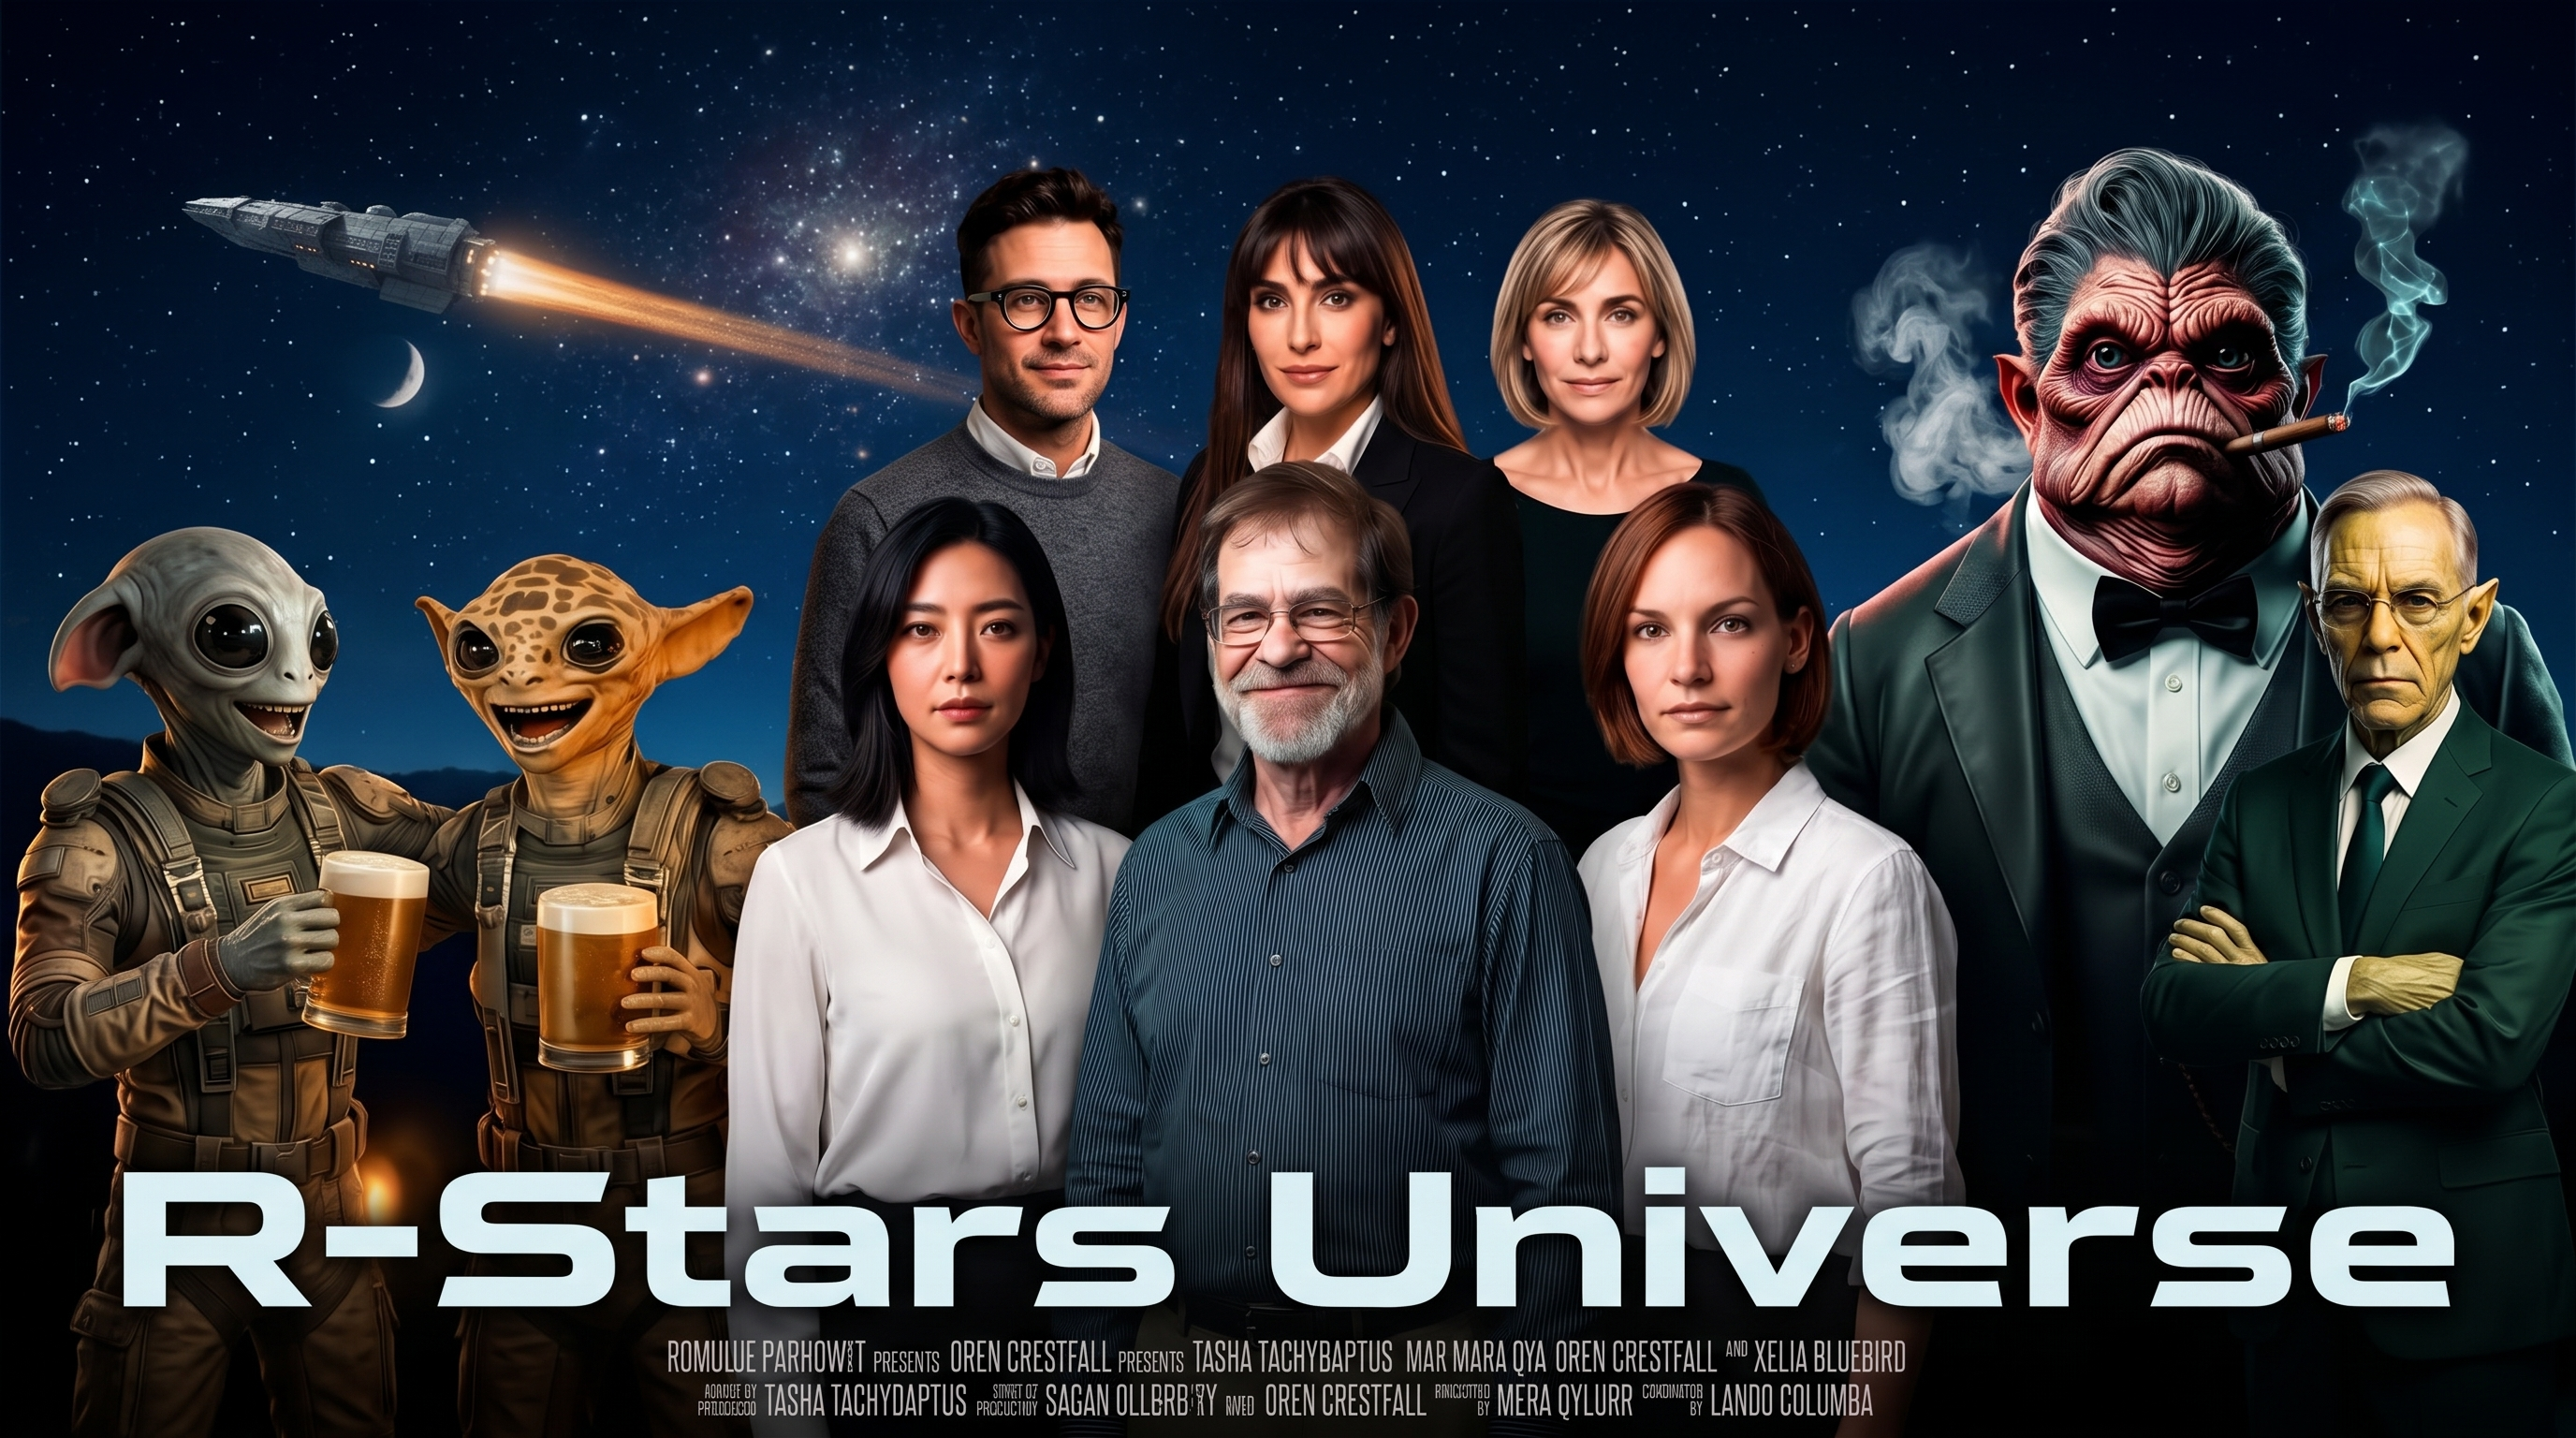
\includegraphics[width=\textwidth]{figuras/Portada_Universo.jpeg}}\par
  \vspace{2.2cm}
  {\sffamily\fontsize{34}{40}\selectfont\bfseries\color{rstars} R-Stars: El Universo\par}
  \vspace{0.6cm}
  {\sffamily\Large\color{rstarsgris} Guía del universo narrativo del proyecto R-Stars\par}
  \vfill
  {\Large Miguel Ángel Tarancón Morán\par}
  \vspace{0.3cm}
  {\normalsize Catedrático de Economía Aplicada\\
   Universidad de Castilla-La Mancha\par}
  \vspace{1.2cm}
\end{titlepage}

\thispagestyle{empty}
\vspace*{\fill}
\begin{small}
\noindent\textbf{R-Stars: El Universo}\\
© 2026 Miguel Ángel Tarancón Morán\par
\medskip
\noindent Esta obra está publicada bajo una licencia Creative Commons
Atribución-NoComercial-SinDerivadas 4.0 Internacional (CC BY-NC-ND 4.0):
\url{https://creativecommons.org/licenses/by-nc-nd/4.0/deed.es}.
Puede descargarse, leerse, imprimirse y compartirse libremente citando
al autor, sin fines comerciales y sin distribuir versiones modificadas.
Véase el apartado \emph{Licencia} al final del libro.\par
\medskip
\noindent Versión en línea, siempre actualizada (con los vídeos):
\url{https://teckel71.github.io/RStarsUniverso-book/}\par
\medskip
\noindent Este PDF se generó el \today.
\end{small}
\clearpage
